\begin{XeClass}{Seekable}
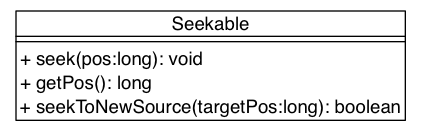
\includegraphics[width=\textwidth]{cdig/Seekable.png}
     
 此接口表示实现该接口的类具有seek方法,具备随机文件读写的能力

    \begin{XeMethod}{}{void}{seek}
         
 从文件的开始位置按给出的偏移量开始查找
 下一次read()会从偏移位置开始查找
 不能查找超过文件尾

    \end{XeMethod}

    \begin{XeMethod}{}{long}{getPos}
         
 返回当前距离文件开始位置的偏移量

    \end{XeMethod}

    \begin{XeMethod}{}{boolean}{seekToNewSource}
         
 查找数据的不同备份
 查找到新的文件返回true,否者返回false

    \end{XeMethod}

\end{XeClass}
